\section{\textbf{\tipsvtwo}} \label{sec:method}

\subsection{Preliminaries} \label{sec:preliminaries}

Our method builds on top of the previous TIPS~\cite{tips_paper} version, a recent vision encoder pretraining method that integrates contrastive image-text learning with self-supervised learning.
In this section, we review the necessary background and introduce the notation used throughout the paper.
Given a collection of image-text pairs $\{(I_k,T_k)\}$, we learn an image encoder $f$ mapping an image $I$ to image embeddings $\{\mathbf e^g,\mathbf e_1,\mathbf e_2,\ldots,\mathbf e_N\}$
and a text encoder $g$ mapping texts $T$ to a text embedding $\mathbf e^t$. Let $f^g(I)=\mathbf e^g$ be the global embedding representation of the entire image and $f(I)=\{\mathbf e_1,\mathbf e_2,\ldots,\mathbf e_N\}$ the patch embeddings corresponding to different image regions. 
$f$ is modeled as a Vision Transformer (ViT)~\citep{dosovitskiy2020vit} and $g$ is modeled as a standard transformer \citep{vaswani2017attention}. The loss is given by $\mathcal{L} = \mathcal{L}_\text{CLIP} + \mathcal{L}_\text{DINO} + \mathcal{L}_\text{iBOT}$, and each component is detailed below.

\noindent\textbf{Image-text contrastive loss.} The first component, $\mathcal{L}_\text{CLIP}$, aligns image and text modalities. Following the approach of CLIP~\citep{radford2021clip}, $\mathcal{L}_\text{CLIP}$ is an InfoNCE~\citep{oord2018infonce} loss that pushes $\mathbf e^g$ and $\mathbf e^t$ close for corresponding images and captions, and far otherwise. TIPS adapts this by introducing two separate CLS global embeddings: one supervised by web alt-text captions for object-centric details, and another supervised by PaliGemma~\citep{beyer2024paligemma} synthetic captions designed to better capture dense spatial relationships. 

\noindent\textbf{Global- and patch-level SSL.}
In addition, TIPS applies two forms of self-supervised losses to boost spatial awareness, using a teacher network $f_t$ that is the exponential moving average (EMA) of the student network $f_s$. In these losses, the teacher network $f_t$ processes the original image $I$, and the student network $f_s$ processes a crop or masked view. Then, these embeddings are projected into a higher ``prototype" dimension by head networks $h_s$ and $h_t$, and the resulting prototypes are supervised to be invariant to these transformations by a cross-entropy loss.
In the global-level self-distillation objective (DINO~\citep{caron2021dino}), the student representations of $M$ local crops $\{I_i\}_{i=1}^M$ are compared to the teacher representation of $I$ on global embeddings:
\begin{equation}
    \label{eq:dino_loss}
        \mathcal{L}_\text{DINO} = - \sum_{i=1}^M  h_t(f_t^g(I))^T \log h_s(f_s^g(I_i))
\end{equation}

\begin{table}[t]
\caption{\small\textbf{Zero-shot segmentation with a large teacher model and its distilled student.} Surprisingly, the TIPS ViT-L model, which is a student distilled from the TIPS ViT-g teacher, significantly surpasses it.}
\vspace{-2mm}
\scriptsize
\centering
{
\begin{tabular}{l c c c c}
\small \multirow{2}{*}{Model} & \multicolumn{4}{c}{Zero-shot Segmentation (mIoU) $\uparrow$} \\
 & PC59 & PC60 & VOC21 & ADE150 \\
\midrule
TIPS ViT-L & \bf{33.5} & \bf{30.4} & \bf{30.5} & \bf{20.8} \\
TIPS ViT-g & 11.4 & 10.8 & 19.7 & 2.6 \\
\end{tabular}
}
\vspace{-0mm}
\label{tab:zeroseg_scale}
\end{table}


\noindent In the patch-level MIM objective (iBOT~\citep{zhou2022ibot}), a random binary mask $m$ is applied to image patches to obtain masked view $I_\text{mask}$ ($m_i=1$ denotes that the $i$-th patch is masked). Then, the student representation of $I_\text{mask}$ is compared to the teacher representation of $I$ on patch embeddings: 
\begin{equation}
    \label{eq:ibot_loss}
        \mathcal{L}_\text{iBOT} = - \sum_{i=1}^N  m_i  h_t(f_t(I)_i)^T \log h_s(f_s(I_\text{mask})_i)
\end{equation}

\begin{figure*}[ht]
    \centering
    \begin{minipage}[c]{0.70\linewidth}
        \vspace{-1mm}
        \scriptsize
        \centering
        {
            \resizebox{1.05\linewidth}{!}{
                \begin{tabular}{l r r c c c c c c}
\small \multirow{2}{*}{Setting} & \multicolumn{2}{c}{Initialization / Update} & Masking Ratio & \multicolumn{4}{c}{Zero-shot Segmentation (mIoU) $\uparrow$} \\
 & Text Encoder & Student Encoder & & PC59 & PC60 & VOC21 & ADE150  \\
\midrule
(1) pretraining & Random / \twemoji{fire}  & Random / \twemoji{fire} & 0.75 & 6.9 & 6.6 & 6.7 & 0.3 \\ 
(2) distillation & Random / \twemoji{fire}  & Random / \twemoji{fire} & 0.75 & 16.0 & 15.4 & 22.5 & 5.9 \\
(3) distillation & Random / \twemoji{fire}  & Random / \twemoji{fire} & 0.5 & 15.5 & 14.5 & 24.0 & 7.0 \\
(4) distillation & Random / \twemoji{fire}  & Random / \twemoji{fire} & 0.0 & \bf{31.4} & \bf{28.6} & \underline{30.8} & \underline{20.0} \\
(5) distillation & Pretrained / \twemoji{fire}  & Random / \twemoji{fire} & 0.0 & \underline{31.1} & \underline{28.5} & \bf{31.9} & \bf{20.5} \\
(6) distillation & Pretrained / \twemoji{snowflake} & Random / \twemoji{fire} & 0.0 & 30.1 & 27.7 & 28.4 & \underline{20.0} \\
(7) distillation & Pretrained / \twemoji{fire}  & Pretrained / \twemoji{fire} & 0.0 & 6.4 & 6.0 & 6.7 & 2.4 \\
\end{tabular}

            }
        }
        \captionof{table}{\textbf{Initialization and masking ablations for distillation.} Comparing TIPS ViT-L models re-trained with different strategies. We highlight \textbf{best} and \underline{second-best} overall. Initialization is either from scratch (``Random") or initialized from the teacher model (``Pretrained"). Update is either training (\twemoji{fire}) or frozen (\twemoji{snowflake}). The results show that removing masking and randomly initializing the student image encoder are critical for achieving strong patch-text alignment.
        }
        \label{tab:init}
    \end{minipage}
    \hfill %
    \begin{minipage}[c]{0.25\linewidth}
        \centering
        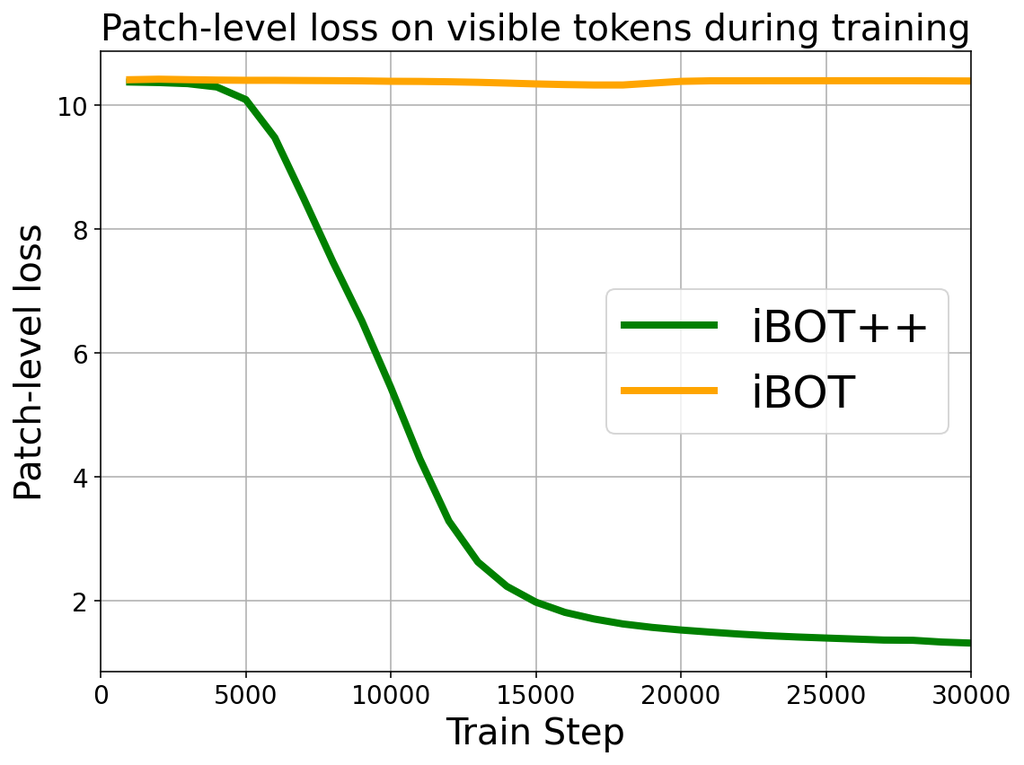
\includegraphics[width=\linewidth]{figures/patch_loss.png}
        \vspace{-6.5mm}
        \caption{
        The decrease in patch-level loss for visible tokens using iBOT++ indicates successful anchoring to the teacher's tokens, which does not happen for iBOT.
        }
        \label{fig:ibot++}
    \end{minipage}
\end{figure*}

\noindent\textbf{Distillation.}
TIPS also distills a family of smaller models with a simple strategy that mirrors the pretraining setup. Distillation only requires two modifications: the teacher network $f_t$ is replaced with a frozen larger teacher instead of an EMA copy of $f_s$, and no mask is applied at the patch-level loss. 

\subsection{Bridging Pretraining and Distillation}
\label{bridge}



In this section, we study the effect of distillation techniques on patch-text alignment. Our main finding is that the patch-level distillation procedure can significantly enhance patch-text alignment, even when utilizing a teacher with poor alignment. To demonstrate this, we begin by evaluating patch-text alignment using standard zero-shot semantic segmentation benchmarks: ADE150~\citep{zhou2017ade20k, zhou2018semanticunderstandingscenesade20k}, Pascal Context (PC59/PC60)~\citep{Mottaghi_2014_CVPR}, and Pascal VOC (VOC21)~\citep{everingham2010pascal}.

As shown in \cref{tab:zeroseg_scale}, the largest pretrained ViT-g TIPS model significantly underperforms the smaller ViT-L student model (which is distilled from the ViT-g) in the task of zero-shot segmentation, reversing the trend of all other tasks reported in \citep{tips_paper}. 
This discrepancy suggests that while the pre-training recipe at the ViT-g scale is highly effective for image-only or global tasks, it fails to induce strong patch-text alignment, a capability apparently gained during distillation. 
To disentangle the factors distinguishing pretraining from distillation, \cref{tab:init} presents ablations using a ViT-L self-distillation baseline. We systematically vary the masking ratio and model initialization/freezing parameters to isolate their individual contributions:
\begin{itemize} 
\item  \textbf{Distillation method:} The models in rows (2-7) are distilled from the frozen ViT-L teacher trained in row (1). These follow the distillation procedure of \citep{tips_paper} described in \cref{sec:preliminaries}, except that the teacher is the same size as the student, to study the setting of distillation in isolation from the effect of a larger teacher. The other differences from vanilla distillation are described row-by-row.

\item \textbf{Masking ratio:} We ablate the effect of masking ratio by lowering it through rows (2-4). In (2), the ratio is the same as vanilla pre-training, and in (4) it is lowered to no masking, which is the ratio in vanilla distillation. Observe that row (2) is the pre-training setting with two key changes: the teacher is frozen and, more importantly, the patch-level loss is also applied to the $25\%$ of unmasked tokens instead of unsupervised as in pre-training. This configuration already yields a significant enhancement in zero-shot segmentation, demonstrating the potential of patch-level distillation for improving patch-text alignment. In contrast, observe that (4) exactly matches the vanilla distillation of \citep{tips_paper}. The increase in patch-text alignment from rows (2-4) as we lower the masking ratio indicates that the loss on visible tokens is critical for achieving improved patch-text alignment during distillation.

\item \textbf{Initialization and freezing:} We ablate the effect of random vs. pre-trained initialization and freezing the text encoder in the remaining rows. We find that the text encoder is less sensitive to initialization in rows (4–6). However, row (7) demonstrates that random initialization is essential for the vision encoder. Initializing distillation with the pre-trained visual encoder as in row (7) completely eliminates the advantage from distillation, reducing it to the performance of the original pre-trained model. This suggests that the model must break away from the pretrained convergence region to learn effectively during distillation.

\end{itemize}

These findings suggest that supervising all patch tokens, rather than just masked ones, is crucial for alignment during distillation. We leverage these insights to formulate a novel pretraining strategy, to be discussed next.
An overview of the final \tipsvtwo pretraining recipe is presented in \cref{fig:block}.


\subsection{iBOT++}
\label{loss_diff}

As discussed in \cref{sec:preliminaries}, both the pretraining and distillation stages of the vision encoder reference method incorporate a patch-level loss.
The pretraining phase employs the iBOT \citep{zhou2022ibot} MIM objective, where the student reconstructs masked tokens by matching the features of a teacher encoder that processes the unmasked image.
For distillation, masking is removed entirely, so both the student and teacher see the unmasked image.


Based on \cref{bridge}, we hypothesize that limiting loss to masked regions discourages preserving local semantics. To resolve this, we propose \textbf{iBOT++}, a modification to iBOT which applies the patch-level loss to all patches, both masked and unmasked.
This simple change represents a significant improvement to the pretraining stage of TIPS.
The improved loss $\mathcal{L}_\text{iBOT++}$  differs from the original $\mathcal{L}_\text{iBOT}$ in \cref{eq:ibot_loss} only in that the loss also applies on visible tokens: 
\begin{equation}
    \label{eq:ibot_plus_loss}
        \mathcal{L}_\text{iBOT++} = - \sum_{i=1}^N   h_t(f_t(I)_i)^T \log h_s(f_s(I_\text{mask})_i)
\end{equation}


While foundational vision encoders~\citep{tips_paper, oquab2024dinov2, siméoni2025dinov3} require high masking ratios (e.g., $75\%$) for successful MIM~\citep{he2022mae} in pre-training, we found in \cref{bridge} that distillation instead benefits substantially from matching student to teacher representations across all tokens without masking. 
iBOT++ operates as an intermediate between these two objectives: we retain the masking mechanism but extend the supervision to visible tokens, requiring the student to align with teacher representations for both masked and unmasked patches. 
Replacing iBOT with iBOT++ in TIPS pretraining yields significant gains in zero-shot segmentation (\cref{tab:fromscratch_distill}), indicating superior patch-text alignment. 
\cref{results} demonstrates that iBOT++ also generally benefits other tasks.

\begin{figure}[t]
    \centering
    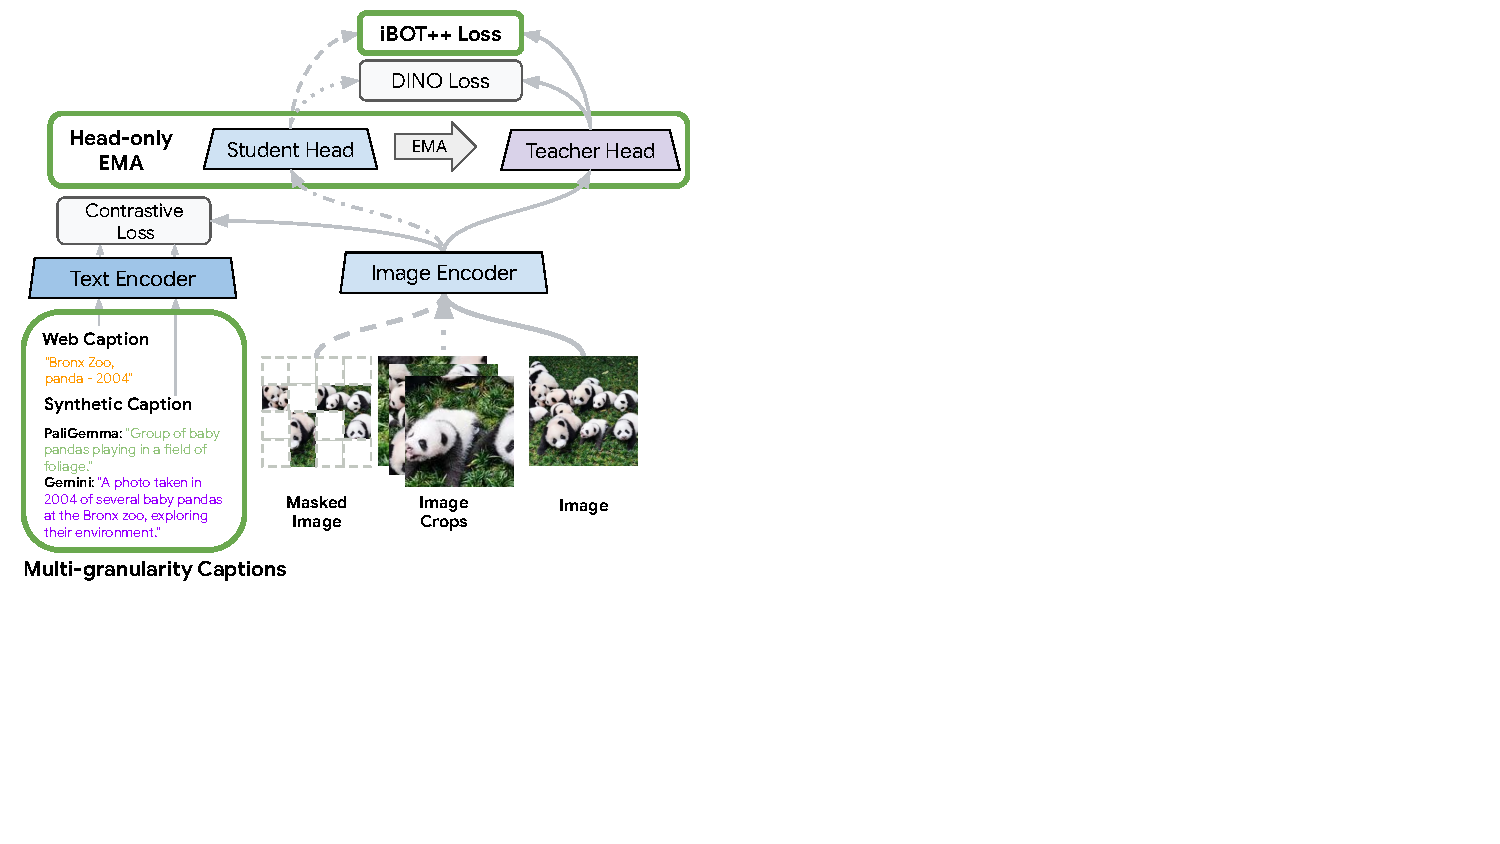
\includegraphics[width=1.0\linewidth]{figures/tipsv2_block.pdf}
    \caption{
    \textbf{\tipsvtwo pretraining overview}. \tipsvtwo introduces $3$ improvements (highlighted in green borders) to the combined contrastive and self-supervised approach to pretrain vision encoders.
    iBOT++ is an enhanced masked image modeling loss.
    Head-only EMA enables memory-efficient self-supervised losses.
    Multi-granularity captions provide a range of possible textual descriptions for images, increasing the robustness of the model.    
    }
    \label{fig:block}
\end{figure}

Note that standard iBOT lacks direct supervision on visible tokens, which allows their representations to behave arbitrarily provided they suffice for reconstructing masked tokens. 
Enforcing alignment on unmasked tokens enables iBOT++ to anchor student patch representations to the teacher's.
This is demonstrated in \cref{fig:ibot++}, which indicates through the proxy of patch-level loss that the representations of visible patches remain poor in iBOT but improve in iBOT++.
Overall, iBOT++ delivers superior performance by simultaneously capturing global context for reconstruction and preserving local semantics.

\subsection{Head-only EMA}
\label{init_diff}

Standard self-distillation ~\citep{caron2021dino, zhou2022ibot, oquab2024dinov2, tips_paper} relies on an EMA teacher network to provide stable targets via temporal ensembling.
Crucially, in the context of SSL-only methods, an EMA teacher with a stop gradient avoids~\citep{grill2020bootstrap} the trivial solution where the prototype representations of student $h_s(f_s(I))$ and teacher $h_t(f_t(I))$ collapse to a constant representation regardless of input $I$. %
This collapse can happen at either the encoder $f_s, f_t$ or at the head $h_s, h_t$.
However, in the context of combined SSL and image-text contrastive learning, the encoders $f_s$ and $f_t$ are already constrained to prevent collapse by the contrastive loss $\mathcal{L}_\text{CLIP}$.
As a result, we propose that it is sufficient to use the EMA teacher only for the head network, and entirely eschew the EMA teacher for the main vision encoder.
That is, we set $f_t = f_s$ and continue only to update $h_t$ by EMA updates from $h_s$. 

Ablations in \cref{results} demonstrate that applying EMA exclusively to the projector head retains the majority of the performance of applying EMA to both head and encoder while significantly reducing resource requirements.
As EMA methods require a second copy of all parameters being averaged during training, this resource-efficient adaptation represents significant savings in memory overhead and training throughput.
For example, on ViT-B, this method reduces training parameters by $42\%$.
Also, note that this design represents a necessary intermediate, as our preliminary experiments find that entirely removing EMA by sharing both the encoder and projector causes severe training instability and performance degradation.


\begin{table}[t]
\caption{\small\textbf{Zero-shot segmentation in pretraining.} Comparing TIPS ViT-g with iBOT or iBOT++ methods, showing significant improvements with our novel iBOT++.}
\vspace{-1mm}
\scriptsize
\centering
{
\begin{tabular}{l c c c c}
\small \multirow{2}{*}{Model} & \multicolumn{4}{c}{Zero-shot Segmentation (mIoU) $\uparrow$} \\
& PC59 & PC60 & VOC21 & ADE150  \\
\midrule
TIPS~\cite{tips_paper} (with iBOT) & 14.2 & 13.4 & 29.1 & 3.5 \\ 
TIPS with iBOT++ & \bf{28.6} & \bf{26.2} & \bf{37.2} & \bf{17.6} \\
\end{tabular}
}
\vspace{-0mm}
\label{tab:fromscratch_distill}
\end{table}
 


\begin{figure}[t]
\begin{center}
   
\includegraphics[width=1.0\linewidth]{figures/captions.pdf}
\end{center}
\vspace{-2mm}
  \caption{
  \textbf{Image captions at different granularities.}
  Besides the alt-text and PaliGemma captions used in previous work, we propose additionally leveraging the more comprehensive Gemini captions, to make our vision encoder more robust.
 }
\label{fig:captions}
\end{figure}

\subsection{Multi-Granularity Text Captions}
\label{multi_caption}

 \cref{fig:captions} illustrates limitations in the alt-text and PaliGemma captions used in~\citep{tips_paper}. 
 For instance, in the panda image, both captions fail to describe the animal's pose (dangling legs and head resting on the branch).
 Similarly, in the illustration example, neither caption identifies the image as a cartoon, a key piece of semantic information. 
 Finally, in the last example, both captions overlook the seasonal context, where the yellow leaves indicate autumn.
 As the vision encoder's learning is directly tied to caption quality, these failures motivate the need for richer, more descriptive captions.

\begin{table*}[t]
\caption{\small\textbf{Ablation studies for \tipsvtwo's pretraining technique}. Ablations are cumulative, running on a fixed schedule of $100$k steps at resolution $224$, for fair comparisons. We highlight the \textbf{best} and \underline{second-best} number of each column.}
\vspace{-2mm}
\scriptsize
\addtolength{\tabcolsep}{0.2em}
\centering
{
\begin{tabular}{l c c c c c c c}
\small \multirow{2}{*}{Model} & Seg. $\uparrow$ & Depth $\downarrow$ & Normals $\downarrow$ & ImageNet $\uparrow$ & I$\rightarrow$T Ret. $\uparrow$ & T$\rightarrow$I Ret. $\uparrow$ & Zero-shot Seg. $\uparrow$ \\
& PASCAL & NYUv2 & NYUv2 & KNN & Flickr & Flickr & ADE150 \\
\midrule
TIPS ViT-g (reproduced)& 82.8 & 0.375 & 23.1 & 83.2 & 92.0 & 81.0 & 3.5 \\
+ iBOT++ & 82.5 & 0.369 & \textbf{22.7} & \textbf{84.4} & 93.9 & \underline{81.7} & 17.6 \\
+ Multi-granularity Captions & \underline{83.7} & \underline{0.354} & \textbf{22.7} & \underline{84.3} & \underline{95.0} & \textbf{85.4} & \underline{18.1} \\
+ Head-only EMA & \textbf{83.8} & \textbf{0.353} & \underline{22.8} & 84.1 & \textbf{95.4} & \textbf{85.4} & \textbf{19.1} \\
\end{tabular}
}
\label{tab:ablation_studies}
\end{table*}


We extend this by generating richer synthetic captions using Gemini Flash \citep{geminiteam2024gemini}, conditioned on the image, alt-text, and PaliGemma captions, as \cref{fig:captions}.
Despite their higher quality, preliminary experiments showed that longer captions underperformed in isolation.
This occurs because overly comprehensive captions trivialize the contrastive loss ($\mathcal{L}_\text{CLIP}$).
The abundance of detail facilitates discrimination within the batch, ultimately hindering the learning of robust representations.
To address this, we randomly alternate between detailed Gemini captions and simpler PaliGemma captions during training to supervise the second CLS token. 
This balances learning difficulty and detail extraction, empirically boosting both dense and global performance.










